\documentclass[border=10pt]{standalone}
\usepackage{tikz,amsmath}
\usetikzlibrary{arrows.meta}

% ========== 配色 ==========
\definecolor{hidFill}{RGB}{199,203,243}
\definecolor{hidLine}{RGB}{52,58,143}
\definecolor{orFill}{RGB}{250,224,180}
\definecolor{orLine}{RGB}{190,110,20}
\definecolor{inFill}{RGB}{183,224,177}
\definecolor{inLine}{RGB}{32,102,32}
\definecolor{outFill}{RGB}{243,199,199}
\definecolor{outLine}{RGB}{143,52,52}

\begin{document}
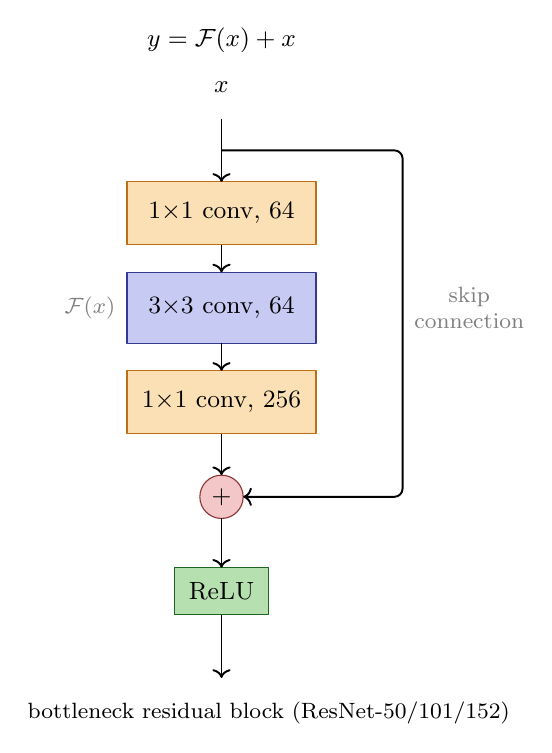
\begin{tikzpicture}[
    font=\small, line join=round,
    every node/.style={inner sep=0pt, outer sep=0pt, align=center},
    conv3/.style={draw=hidLine, fill=hidFill, minimum width=2.4cm, minimum height=.9cm},
    conv1/.style={draw=orLine, fill=orFill, minimum width=2.4cm, minimum height=.8cm},
    relu/.style={draw=inLine, fill=inFill, minimum width=1.2cm, minimum height=.6cm},
    add/.style={circle, draw=outLine, fill=outFill, minimum size=.55cm},
    arr/.style={->, line width=.7pt, rounded corners=3pt}
  ]

  % ================= 瓶颈残差块 =================
  \node at (0,7.8) {$y=\mathcal{F}(x)+x$};          % 公式放顶部
  \node (xin) at (0,7.2) {$x$};
  \node[conv1] (c1) at (0,5.6) {1$\times$1 conv, 64};
  \node[conv3] (c2) at (0,4.4) {3$\times$3 conv, 64};
  \node[conv1] (c3) at (0,3.2) {1$\times$1 conv, 256};
  \node[add]   (ad) at (0,2.0) {+};
  \node[relu]  (r2) at (0,0.8) {ReLU};
  % 主路（x 与箭头之间留空）
  \draw[arr] (0,6.8) -- (c1);
  \coordinate (s) at (0,6.4);
  \draw[arr] (c1) -- (c2);
  \draw[arr] (c2) -- (c3);
  \draw[arr] (c3) -- (ad);
  \draw[arr] (ad) -- (r2);
  \draw[arr] (r2) -- (0,-0.3);
  % 跳跃连接（第一段水平）
  \draw[arr] (s) -- (2.3,6.4) -- (2.3,2.0) -- (ad.east);
  % 侧边标注（横排；skip 拆两行）
  \node[font=\footnotesize, text=gray, anchor=east] at (-1.35,4.4) {$\mathcal{F}(x)$};
  \node[font=\footnotesize, text=gray, anchor=west] at (2.45,4.4) {skip\\connection};
  \node[font=\footnotesize] at (0.6,-0.75) {bottleneck residual block (ResNet-50/101/152)};

\end{tikzpicture}
\end{document}